% Universidade Federal do Rio Grande do Norte
% Programa de Pos-Graduacao em Engenharia Eletrica e de Computacao
% Lista 1 - Questao 4
% Autores: Anna Giselle Camara Dantas Ribeiro
%          Cristiano Gurgel de Castro
%          Diogo Leite Reboucas
%          Thiago Medeiros Barros

% Revisado em 15/06/2010 12:38 por crisgc

  \chapter*{Questão 4}
% Enunciado
\noindent {\it Seja o sistema da Fig. \ref{fig:q4:sist}. Considerando $G(s) =
\frac{2e^{-s}}{s+0.25}$, pede-se: }

\begin{itemize}
    \item[a)] {\it projetar um controlador PI de forma que o desempenho do
              sistema em malha fechada não apresente sobre-sinal. Simule a 
              resposta no \Matlab.}
    \item[b)] {\it Considerando o sistema com o controlador projetado no item a
              e considerando $G_d(s) = 1$, projetar um controlador feedforward 
              (realizável) e avaliar o desempenho do sistema completo utilizando
              o \Matlab.}
\end{itemize}

\begin{figure}[H]
\centering
    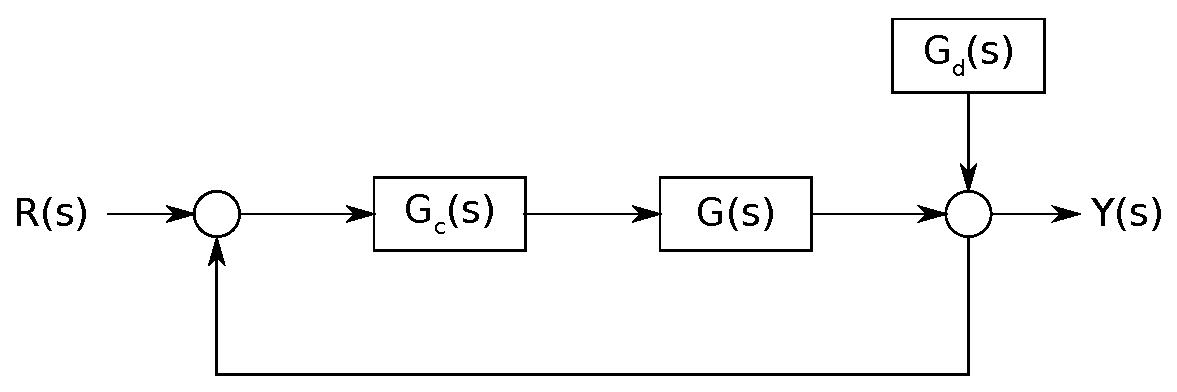
\includegraphics[width=0.65\textwidth]{imgs/questao4/sistema}
    \caption{Diagrama de blocos do sistema.}
    \label{fig:q4:sist}
\end{figure}

% Resolução
\vspace{0.5cm}

\noindent{\bf Resolução:}

\vspace{0.25cm}

% Parte a
O controlador PI foi projetado utilizando o método tradicional, desconsiderando
o atraso do sistema, ou seja, separando o termo $e^{-s}$ do restante da função
de transferência, como pode ser visto na Fig. \ref{fig:q4:projetoPI}.
Definiu-se então $G'(s)$, como sendo a função de transferência sem o atraso de
transporte, ou seja:

\begin{flalign}
G'(s) = \frac{2}{s+0.25} \label{eq:q4:glinha}
\end{flalign}

\begin{figure}[htb]
\centering
\scalebox{0.7}{\begin{picture}(0,0)%
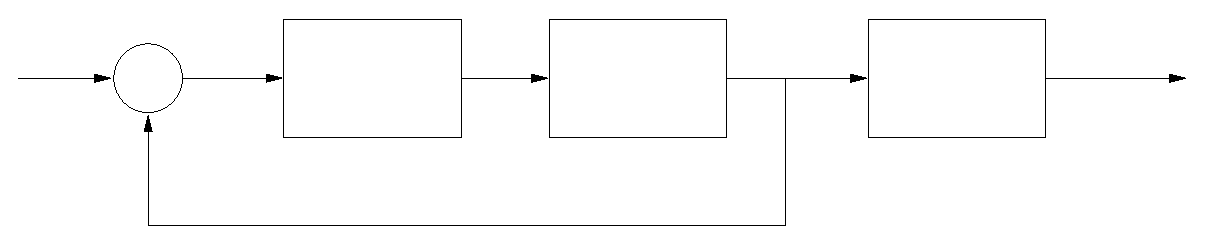
\includegraphics{./imgs/questao4/projetoPI.eps}%
\end{picture}%
\setlength{\unitlength}{4144sp}%
%
\begingroup\makeatletter\ifx\SetFigFont\undefined%
\gdef\SetFigFont#1#2#3#4#5{%
  \reset@font\fontsize{#1}{#2pt}%
  \fontfamily{#3}\fontseries{#4}\fontshape{#5}%
  \selectfont}%
\fi\endgroup%
\begin{picture}(8934,1599)(2914,-3448)
\put(3241,-2176){\makebox(0,0)[b]{\smash{{\SetFigFont{12}{14.4}{\familydefault}{\mddefault}{\updefault}{\color[rgb]{0,0,0}$R(s)$}%
}}}}
\put(5626,-2356){\makebox(0,0)[b]{\smash{{\SetFigFont{12}{14.4}{\familydefault}{\mddefault}{\updefault}{\color[rgb]{0,0,0}$G_c(s)$}%
}}}}
\put(3511,-2536){\makebox(0,0)[b]{\smash{{\SetFigFont{12}{14.4}{\familydefault}{\mddefault}{\updefault}{\color[rgb]{0,0,0}$+$}%
}}}}
\put(4096,-2716){\makebox(0,0)[b]{\smash{{\SetFigFont{12}{14.4}{\familydefault}{\mddefault}{\updefault}{\color[rgb]{0,0,0}$-$}%
}}}}
\put(7651,-2356){\makebox(0,0)[b]{\smash{{\SetFigFont{12}{14.4}{\familydefault}{\mddefault}{\updefault}{\color[rgb]{0,0,0}$\frac{2}{s+0.25}$}%
}}}}
\put(10081,-2356){\makebox(0,0)[b]{\smash{{\SetFigFont{12}{14.4}{\familydefault}{\mddefault}{\updefault}{\color[rgb]{0,0,0}$e^{-s}$}%
}}}}
\put(8911,-2131){\makebox(0,0)[b]{\smash{{\SetFigFont{12}{14.4}{\familydefault}{\mddefault}{\updefault}{\color[rgb]{0,0,0}$Y'(s)$}%
}}}}
\put(11341,-2131){\makebox(0,0)[b]{\smash{{\SetFigFont{12}{14.4}{\familydefault}{\mddefault}{\updefault}{\color[rgb]{0,0,0}$Y(s)$}%
}}}}
\end{picture}%
}
\caption{Projeto de controlador desconsiderando o atraso de transporte.}
\label{fig:q4:projetoPI}
\end{figure}

Primeiramente, analisou-se o sistema em malha fechada sem nenhum controlador ou
seja $G'_c(s) = 1$. O comportamento foi considerado aceitável uma vez que a
saída possui erro de regime aproximadamente nulo e tem uma constante de tempo
razoável (menos de $1$s), conforme Fig.  \ref{fig:q4:saida_mf}. O controlador PI
está, então, adequadamente empregado já que tem por objetivo na sua definição a
melhora do erro de regime.

\begin{figure}[htb]
\centering
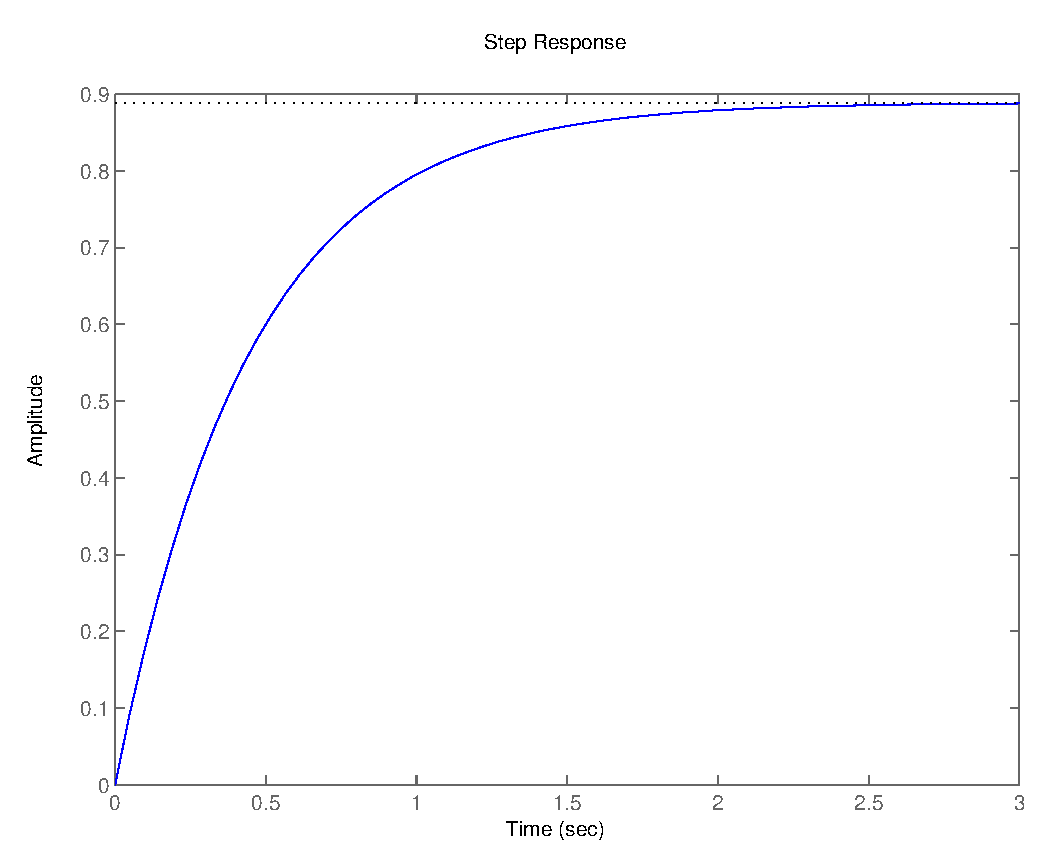
\includegraphics[width=0.65\textwidth]{imgs/questao4/saida_mf}
\caption{Saída do sistema sem o controlador}
\label{fig:q4:saida_mf}
\end{figure}

O requisito do sistema projetado foi a não-presença do sobre-sinal
(\emph{overshoot}). Dessa forma os polos de $G'_c(s)G'(s)$ não devem possuir
parte imaginária, o que significaria oscilações no sinal de saída. Segundo
\citeasnoun{Araujo}, o controlador PI tem a seguinte função de transferência:

\begin{flalign*}
G'_c(s) = k_p + \frac{k_i}{s} = \frac{k_c(s+z)}{s} 
\end{flalign*}

Logo o controlador adiciona um polo na origem e um zero. Para não afetar
demasiadamente as características do transitório, decidiu-se por posicionar o
zero do controlador antes do polo do sistema $G'(s)$, conforme Eq.
\ref{eq:q4:glinha}, ou seja $|z| < 0.25$. O sistema foi simulado com o seguinte
controlador:

\begin{flalign}
G'_c(s) = \frac{s+0.2}{s} \label{eq:q4:glinha_c}
\end{flalign}

\noindent e os resultados obtidos na simulação podem ser visualizados na Fig.
\ref{fig:q4:saida_comp_mf}. O diagrama do lugar geométrico das raízes para o
sistema com o controlador pode ser visualizado na Fig. \ref{fig:q4:rlocus_cmf}.

\begin{figure}[htb]
\centering
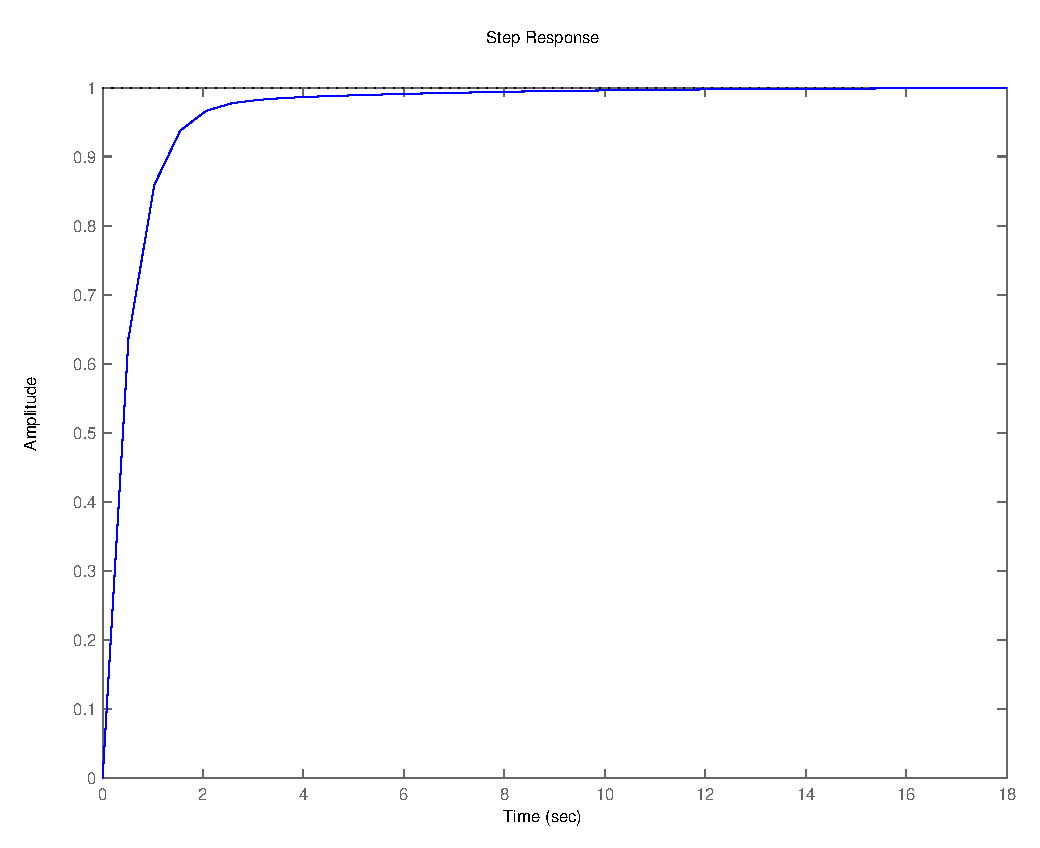
\includegraphics[width=0.65\textwidth]{imgs/questao4/saida_comp_mf}
\caption{Saída do sistema com o controlador projetado $G'_c(s) =
\frac{s+0.2}{s}$.}
\label{fig:q4:saida_comp_mf}
\end{figure}

\begin{figure}[H]
\centering
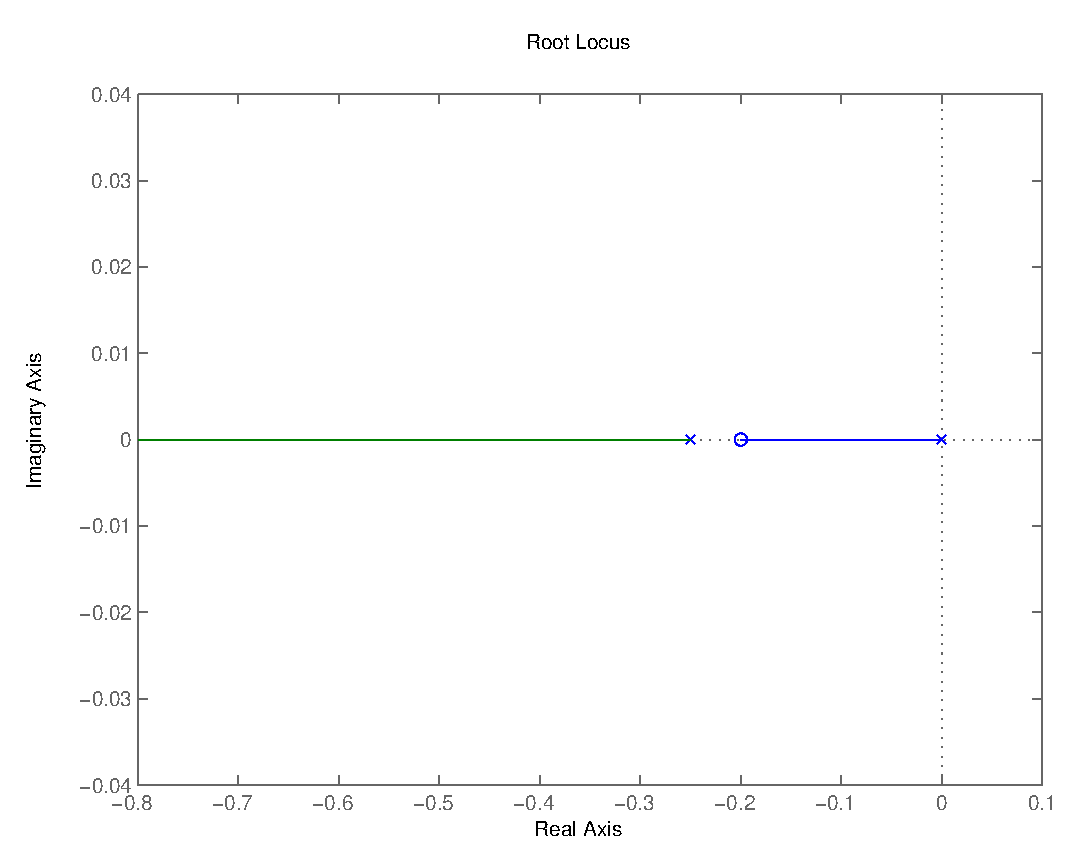
\includegraphics[width=0.65\textwidth]{imgs/questao4/rlocus_cma}
\caption{Lugar das raízes para $G'_c(s)G'(s) = \frac{0.4+2s}{0.25s+s^{2}}$.}
\label{fig:q4:rlocus_cmf}
\end{figure}

A função de transferência de malha fechada para do sistema com o controlador,
juntamente com o valor de $\omega_n$ e $\zeta$ é portanto:

\begin{eqnarray}
G'_{\text{MF}}(s) = \frac{G'_c(s)G'(s)}{1+G'_c(s)G'(s)} =
                    \frac{0.4+2s}{0.4+2.25s+s^{2}}
\end{eqnarray}

\noindent tal que $\omega_n \approx 0.632$ e $\zeta \approx 1.779$.

De acordo com \citeasnoun{Medeiros}, percebe-se que o sistema é sobreamortecido,
já que $\zeta > 1$, portanto a resposta não apresenta o sobressinal. Simulou-se
através do \Simulink\ o desempenho do compensador PI projetado no controle
do sistema $G(s)$ original, ou seja, com o atraso de transporte. O desempenho
foi completamente insatisfatório: o sistema tornou-se instável, conforme Fig.
\ref{fig:q4:saida_cont_dt}. 

\begin{figure}[htb]
\centering
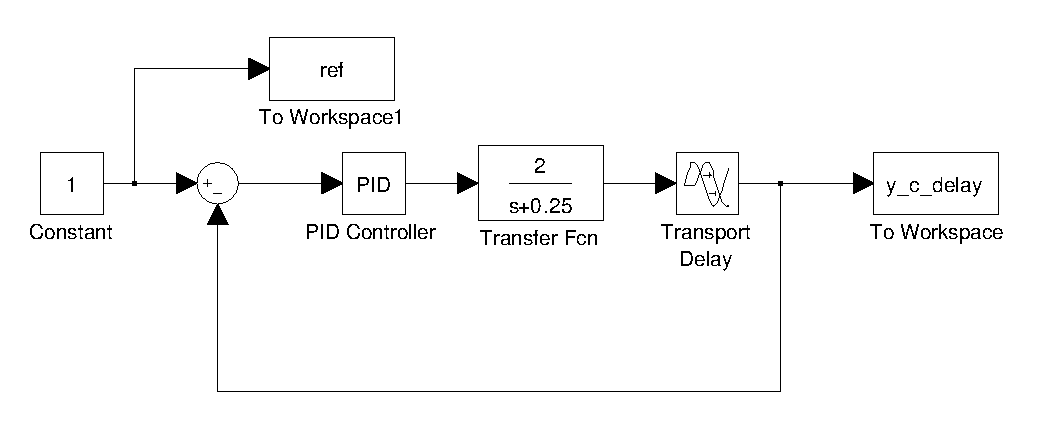
\includegraphics[width=0.65\textwidth]{imgs/questao4/sist_cont_dt}
\caption{Sistema com atraso controlado pelo PI.}
\label{fig:q4:sist_cont_dt}
\end{figure}

\begin{figure}[htb]
\centering
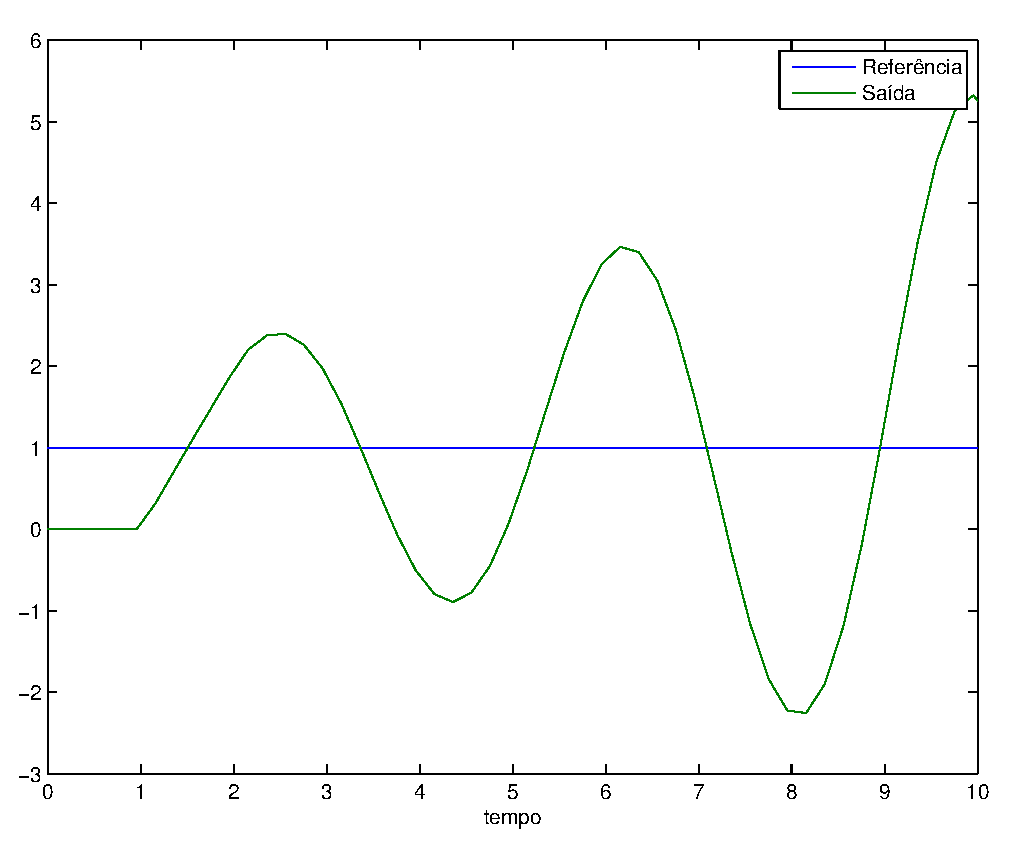
\includegraphics[width=0.65\textwidth]{imgs/questao4/saida_cont_dt}
\caption{Resposta do sistema da Fig. \ref{fig:q4:sist_cont_dt}.}
\label{fig:q4:saida_cont_dt}
\end{figure}

Foi adotado então o preditor de Smith, o qual implementa um tipo de predição
baseado no modelo e possibilita ao controlador projetado agir baseado na
predição $y'(t + L)$, onde $L$ é o atraso de transporte, ou seja, permite ao
controlador agir no sistema como se não houvesse atraso de transporte
\cite{Haegglund1996}. \citeasnoun{Haegglund1996} também justifica porque o tipo
de controlador normalmente usado com preditor de Smith é o PI. O sistema
utilizado para a implementação do preditor bem como o resultado obtido são
mostrados nas Figs. \ref{fig:q4:sist_smith} e \ref{fig:q4:saida_smith}. É
importante ressaltar que nesse preditor foi utilizada uma função de
transferência para predição $\hat{G}(s) = \frac{2}{s+0.25}$ igual, portanto, ao
sistema sem o atraso.

\begin{figure}[htb]
\centering
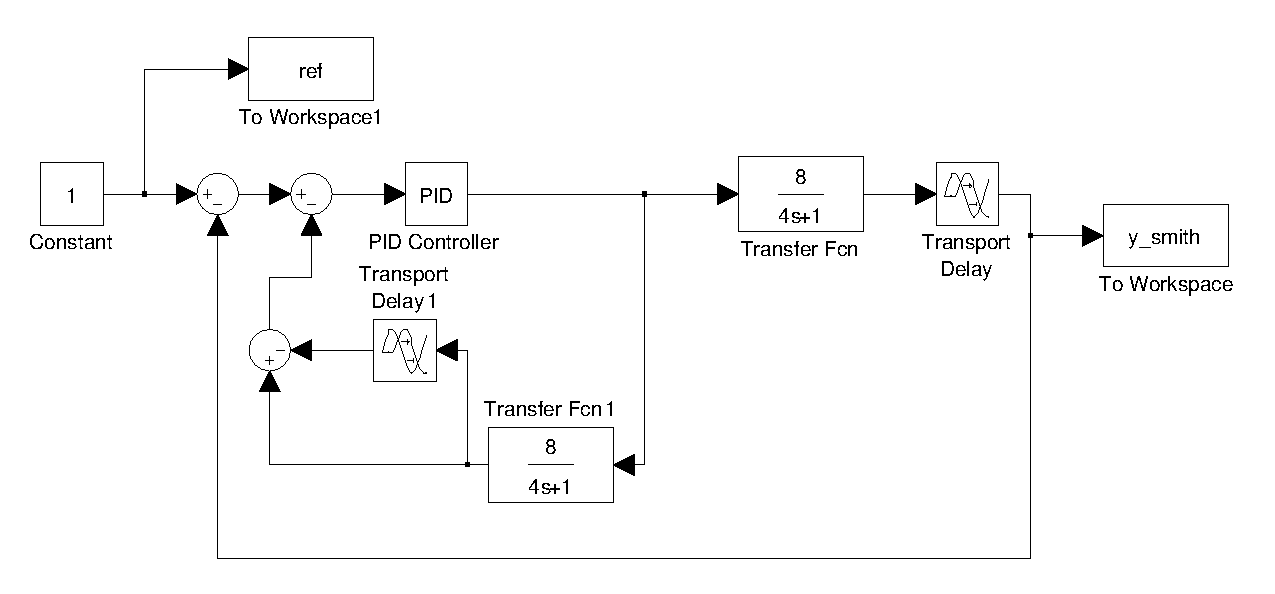
\includegraphics[width=0.75\textwidth]{imgs/questao4/sist_smith}
\caption{Preditor de Smith.}
\label{fig:q4:sist_smith}
\end{figure}

\begin{figure}[htb]
\centering
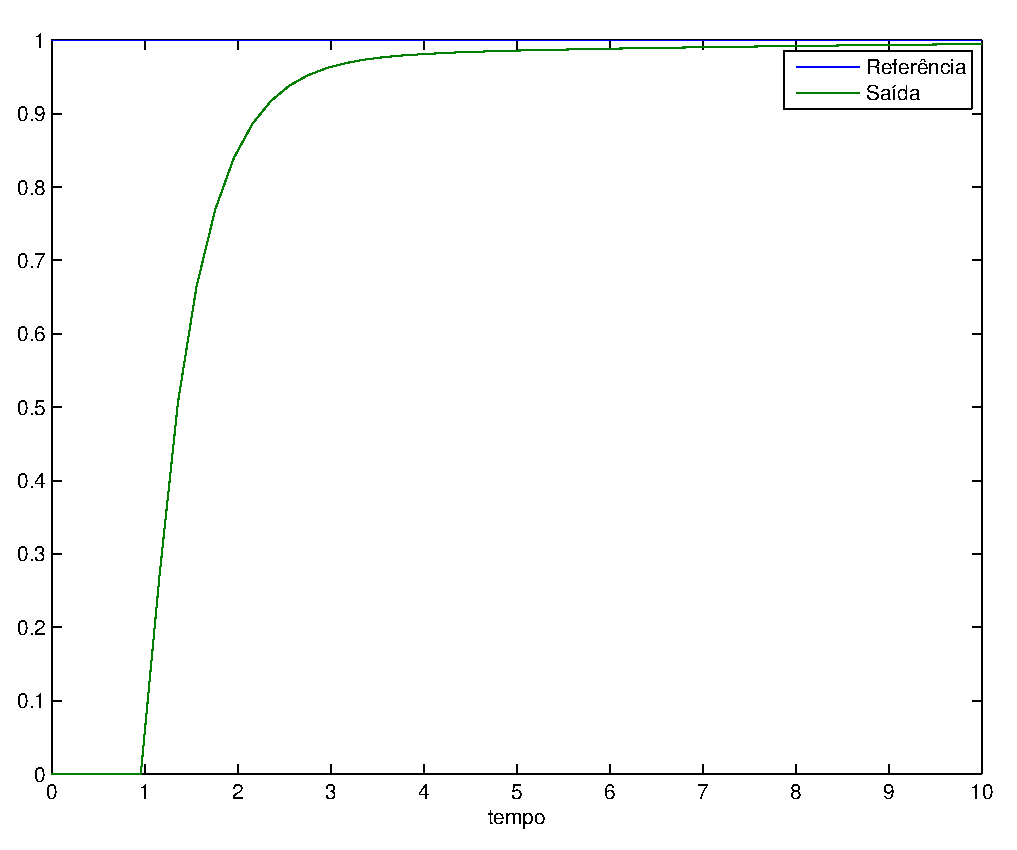
\includegraphics[width=0.65\textwidth]{imgs/questao4/saida_smith}
\caption{Resposta ao controlador com preditor da Fig. \ref{fig:q4:sist_smith}.}
\label{fig:q4:saida_smith}
\end{figure}

Foi analisado também o comportamento do preditor quando o sistema utilizado para
predição não corresponde exatamente ao processo simulado ou seja $\hat{G}(s)
\neq G'(s)$, conforme Fig. \ref{fig:q4:sist_smith_diff}. Apesar de ter
apresentado um baixo e indesejável sobressinal, o resultado foi razoável,
conforme Fig. \ref{fig:q4:saida_smith_diff}, o que mostra a boa adequação do
preditor mesmo com estimativas grosseiras da função de transferência do sistema
original. Escolheu-se para a continuação da questão o sistema tal que
$\hat{G}(s) = G'(s)$. A função de transferência final do controlador é,
portanto: 

\begin{flalign}
G_c(s) = \frac{G'_c(s)}{1 + G'_c(s)(1 - e^{-s})\hat{G}(s)} =
\frac{G'_c(s)}{1 + G'_c(s)(1 - e^{-s})G'(s)} \label{eq:q4:g_c}
\end{flalign}

\begin{figure}[htb]
\centering
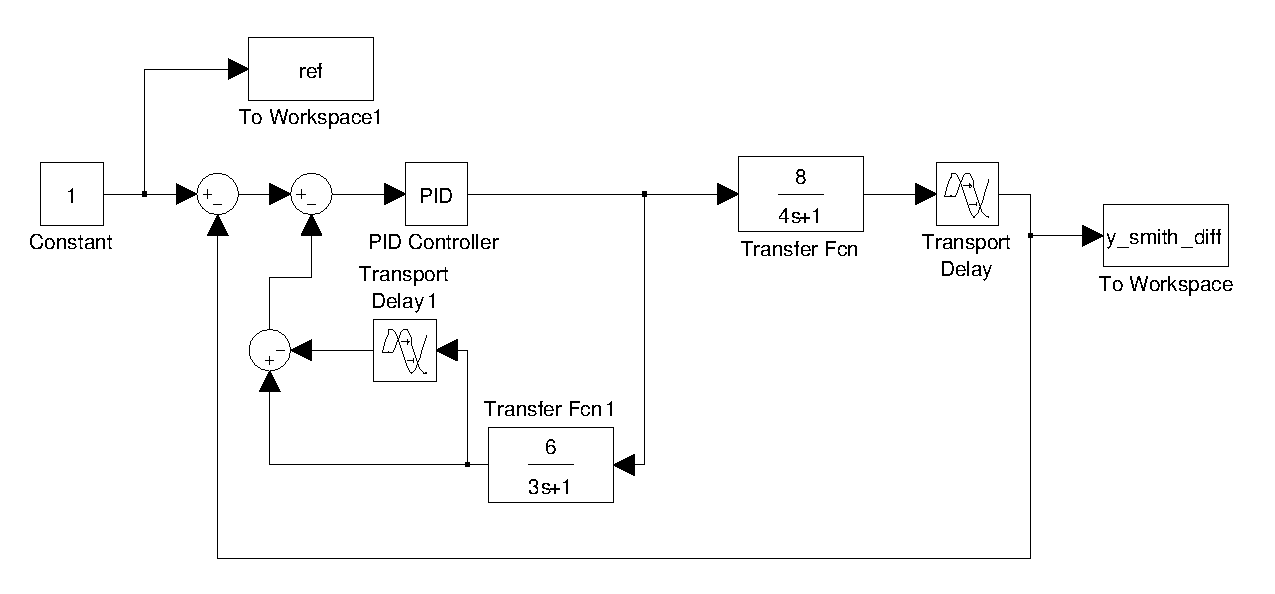
\includegraphics[width=0.65\textwidth]{imgs/questao4/sist_smith_diff}
\caption{Preditor de Smith com $G'(s) = \frac{6}{3s + 1}$.}
\label{fig:q4:sist_smith_diff}
\end{figure}

\begin{figure}[htb]
\centering
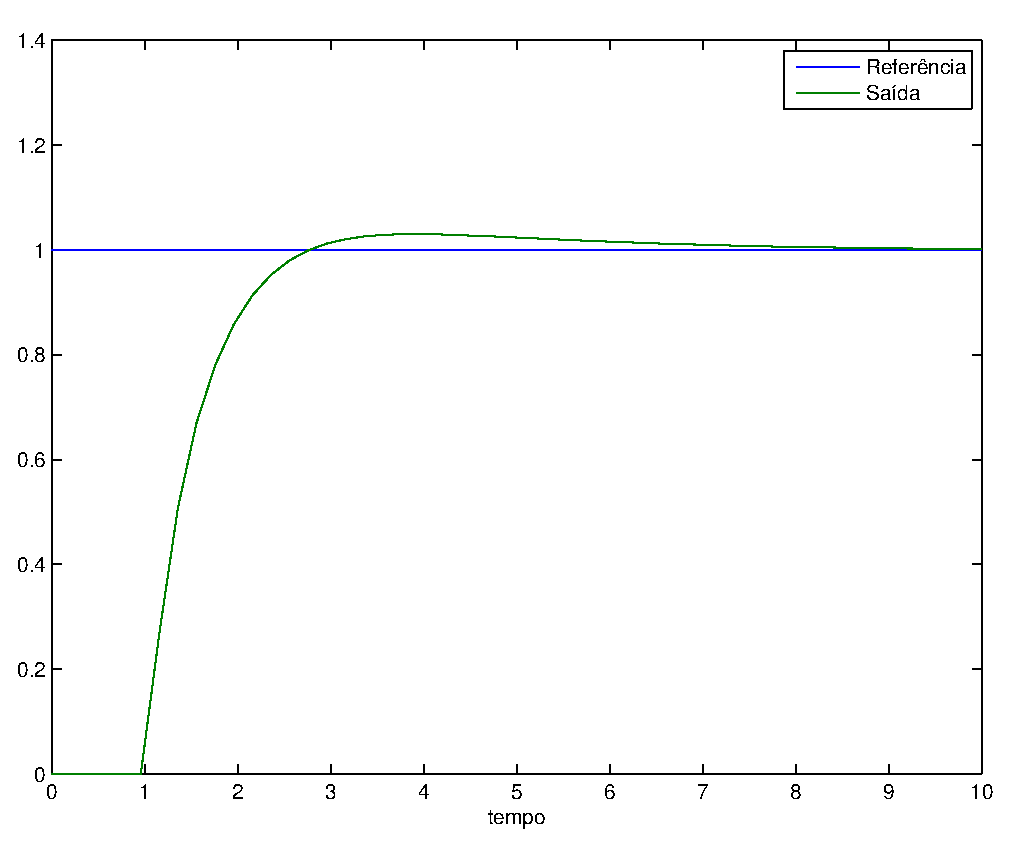
\includegraphics[width=0.65\textwidth]{imgs/questao4/saida_smith_diff}
\caption{Resposta ao controlador com preditor da Fig.
\ref{fig:q4:sist_smith_diff}.}
\label{fig:q4:saida_smith_diff}
\end{figure}

% Parte b

% Considerações sobre Gff(s)
Projetado o controlador PI, analisou-se então o acréscimo do controle {\it
feedforward} ($G_\text{ff}(s)$) ao processo, conforme Fig. \ref{fig:q4:sist_ff}.
Através da análise da figura, com o intuito de cancelar efeito do ruído, tem-se
que:

\begin{flalign*}
G'_\text{ff}(s) & = \frac{G_d(s)}{\underbrace{G_c(s)}_{\text{Eq.
\ref{eq:q4:g_c}}}G(s)} = \frac{1 + G'(s)G'_c(s) -
e^{-s}G'(s)G'_c(s)}{G'(s)G'_c(s)e^{-s}} \\
& = \frac{1 + G'(s)G'_c(s)}{G'(s)G'_c(s)}e^{s} - 1
\end{flalign*}

A partir de $G'_\text{ff}(s)$, pode-se notar que o compensador ideal é irrealizável,
já que envolve tanto um retorno no tempo $e^{s}$, quanto um impulso unitário $1$. Isso
poderia ser previamente notado, sem nenhum cálculo de função de transferência,
através da análise de duas características do sistema:

\begin{itemize}
\item o distúrbio ($D(s)$) atua no sistema instantaneamente, já que $G_d(s) =
1$;
\item qualquer ação na variável manipulada do sistema demorará um tempo $\tau =
1$ para ser refletida na saída, onde $\tau$ é o chamado atraso de transporte do sistema.
\end{itemize}

\begin{figure}[htb]
\centering
\scalebox{0.7}{\begin{picture}(0,0)%
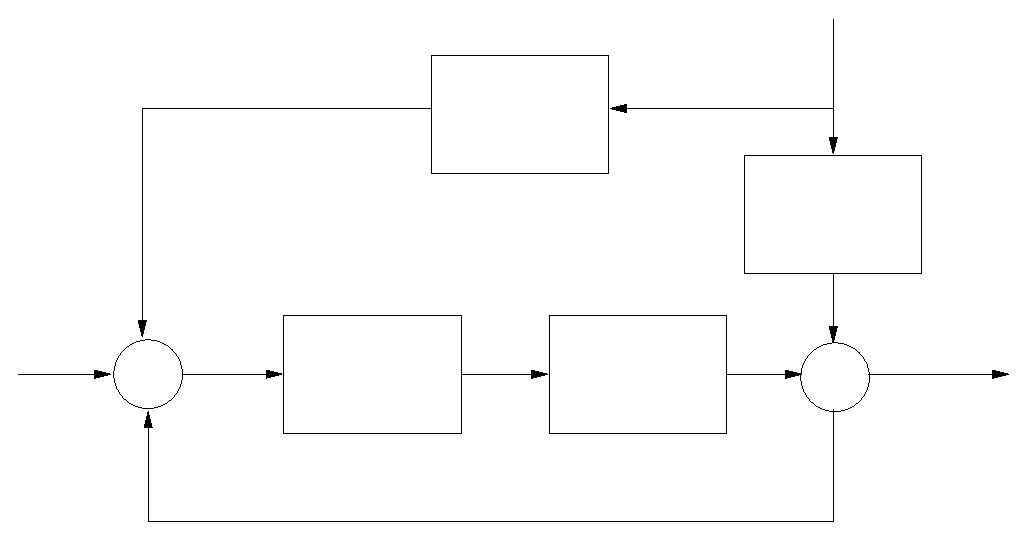
\includegraphics{./imgs/questao4/sist_ff.eps}%
\end{picture}%
\setlength{\unitlength}{4144sp}%
%
\begingroup\makeatletter\ifx\SetFigFont\undefined%
\gdef\SetFigFont#1#2#3#4#5{%
  \reset@font\fontsize{#1}{#2pt}%
  \fontfamily{#3}\fontseries{#4}\fontshape{#5}%
  \selectfont}%
\fi\endgroup%
\begin{picture}(7584,3849)(2914,-3448)
\put(3241,-2176){\makebox(0,0)[b]{\smash{{\SetFigFont{12}{14.4}{\familydefault}{\mddefault}{\updefault}{\color[rgb]{0,0,0}$R(s)$}%
}}}}
\put(5626,-2356){\makebox(0,0)[b]{\smash{{\SetFigFont{12}{14.4}{\familydefault}{\mddefault}{\updefault}{\color[rgb]{0,0,0}$G_c(s)$}%
}}}}
\put(3511,-2536){\makebox(0,0)[b]{\smash{{\SetFigFont{12}{14.4}{\familydefault}{\mddefault}{\updefault}{\color[rgb]{0,0,0}$+$}%
}}}}
\put(4096,-2716){\makebox(0,0)[b]{\smash{{\SetFigFont{12}{14.4}{\familydefault}{\mddefault}{\updefault}{\color[rgb]{0,0,0}$-$}%
}}}}
\put(7651,-2356){\makebox(0,0)[b]{\smash{{\SetFigFont{12}{14.4}{\familydefault}{\mddefault}{\updefault}{\color[rgb]{0,0,0}$G(s)$}%
}}}}
\put(9136,-1141){\makebox(0,0)[b]{\smash{{\SetFigFont{12}{14.4}{\familydefault}{\mddefault}{\updefault}{\color[rgb]{0,0,0}$G_d(s)$}%
}}}}
\put(6751,-331){\makebox(0,0)[b]{\smash{{\SetFigFont{12}{14.4}{\familydefault}{\mddefault}{\updefault}{\color[rgb]{0,0,0}$G_{ff}(s)$}%
}}}}
\put(8686,-2491){\makebox(0,0)[b]{\smash{{\SetFigFont{12}{14.4}{\familydefault}{\mddefault}{\updefault}{\color[rgb]{0,0,0}$+$}%
}}}}
\put(9361,-1996){\makebox(0,0)[b]{\smash{{\SetFigFont{12}{14.4}{\familydefault}{\mddefault}{\updefault}{\color[rgb]{0,0,0}$+$}%
}}}}
\put(4051,-1951){\makebox(0,0)[b]{\smash{{\SetFigFont{12}{14.4}{\familydefault}{\mddefault}{\updefault}{\color[rgb]{0,0,0}$-$}%
}}}}
\put(10081,-2131){\makebox(0,0)[b]{\smash{{\SetFigFont{12}{14.4}{\familydefault}{\mddefault}{\updefault}{\color[rgb]{0,0,0}$Y(s)$}%
}}}}
\put(9586,-16){\makebox(0,0)[b]{\smash{{\SetFigFont{12}{14.4}{\familydefault}{\mddefault}{\updefault}{\color[rgb]{0,0,0}$D(s)$}%
}}}}
\end{picture}%
}
\caption{Projeto de controlador desconsiderando o atraso de transporte.}
\label{fig:q4:sist_ff}
\end{figure}

Com isso, qualquer ruído detectado em um determinado momento, somente poderá a ser
compensado após o atraso de transporte do sistema, portanto o cancelamento de ruído
perfeito não é possível, o que se reflete em um $G'_\text{ff}(s)$ irrealizável. 

% Realizando G_ff
A partir do modelo ideal $G'_\text{ff}(s)$, $G_\text{ff}(s)$ foi projetado eliminando-se o
termo $e^{s}$, assim sendo:

\begin{flalign*}
G_\text{ff}(s) & = \frac{1 + G'(s)G'_c(s)}{G'(s)G'_c(s)}\cancel{e^{s}} - 1 =
\frac{1}{\underbrace{G'(s)}_{\text{Eq.
\ref{eq:q4:glinha}}}\underbrace{G'_c(s)}_{\text{Eq. \ref{eq:q4:glinha_c}}}}
\cancel{+ 1 - 1} = \frac{s(s+0.25)}{2(s+0.2)} \\
& = \frac{1}{2}\frac{s^2 + 0.25s}{s + 0.2}
\end{flalign*}

Observa-se que o número de zeros supera o de polos no sistema. Para contornar o
problema adicionou-se em série dois filtros (passa-baixa) na equação de
transferência $G_\text{ff}(s)$, foram testados dois tipos de filtros $F_1(s) =
\frac{1}{s+1}$ e $F_{10}(s) = \frac{10}{s+10}$, esses filtros possuem ganho
estático $1$ e não influenciam o regime do sistema. 

Analisou-se o comportamento da resposta de três sistemas. O primeiro deles sem o
controle {\it feedforward}, cujos resultados podem ser observados na Fig.
\ref{fig:q4:sist_ruido}.

O segundo dado pela função de transferência $G_{\text{ff}_1}(s)$ apresentada na
Eq. \ref{eq:q4:g_ff1}, cujos resultados podem ser observados na Fig.
\ref{fig:q4:sist_ruido_ff1}.

\begin{flalign}
F_1(s) & = \frac{1}{s+1} \nonumber \\
G_{\text{ff}_1} & = G_\text{ff}(s)F_1(s)F_1(s) = \frac{1}{2}\frac{s^2 + 0.25s}{s +
0.2}\frac{1}{s+1}\frac{1}{s+1} = 0.5\frac{0.25s+s^{2}}{0.2+1.4s+2.2s^{2}+s^{3}}
\label{eq:q4:g_ff1}
\end{flalign}

Por fim, o terceiro dado pela função de transferência $G_{\text{ff}_{10}}(s)$
apresentada na Eq. \ref{eq:q4:g_ff10}, cujos resultados podem ser observados na
Fig. \ref{fig:q4:sist_ruido_ff10}. 

\begin{flalign}
F_{10}(s) & = \frac{10}{s+10} \nonumber \\
G_{\text{ff}_{10}} & = G_\text{ff}(s)F_{10}(s)F_{10}(s) = 
                       \frac{1}{2}\frac{s^2 + 0.25s}{s +0.2}\frac{10}{s+10}
                       \frac{10}{s+10} = 50\frac{s^{2}+0.25s}
                                                {s^{3}+20.2s^{2}+104s+20}
\label{eq:q4:g_ff10}
\end{flalign}

O tipo de ruído utilizado foi um sinal tipo degrau unitário agindo a partir de
$t_r = 5$. Os resultados para os três sistemas estão apresentados nas Figs.
\ref{fig:q4:saida_ruido}, \ref{fig:q4:saida_ruido_ff1} e
\ref{fig:q4:saida_ruido_ff10}, respectivamente.

\begin{figure}[htb]
\centering
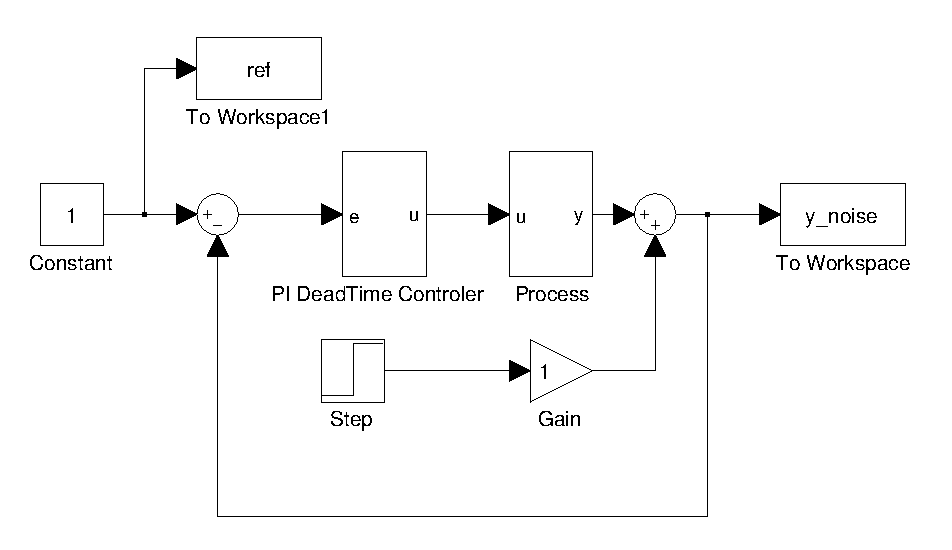
\includegraphics[width=0.75\textwidth]{imgs/questao4/sist_ruido}
\caption{Sistema com ruído na saída sem compensação {\it feedforward}.}
\label{fig:q4:sist_ruido}
\end{figure}

\begin{figure}[htb]
\centering
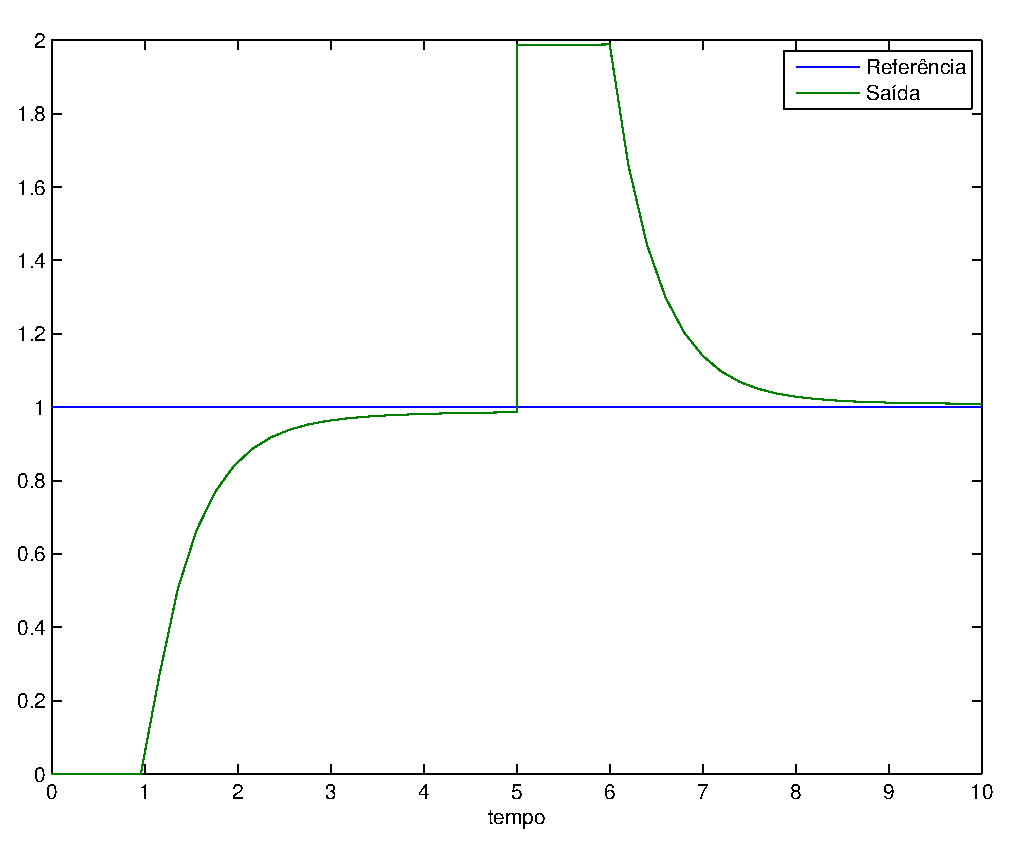
\includegraphics[width=0.65\textwidth]{imgs/questao4/saida_ruido}
\caption{Resposta do sistema da Fig. \ref{fig:q4:sist_ruido}.}
\label{fig:q4:saida_ruido}
\end{figure}

\begin{figure}[htb]
\centering
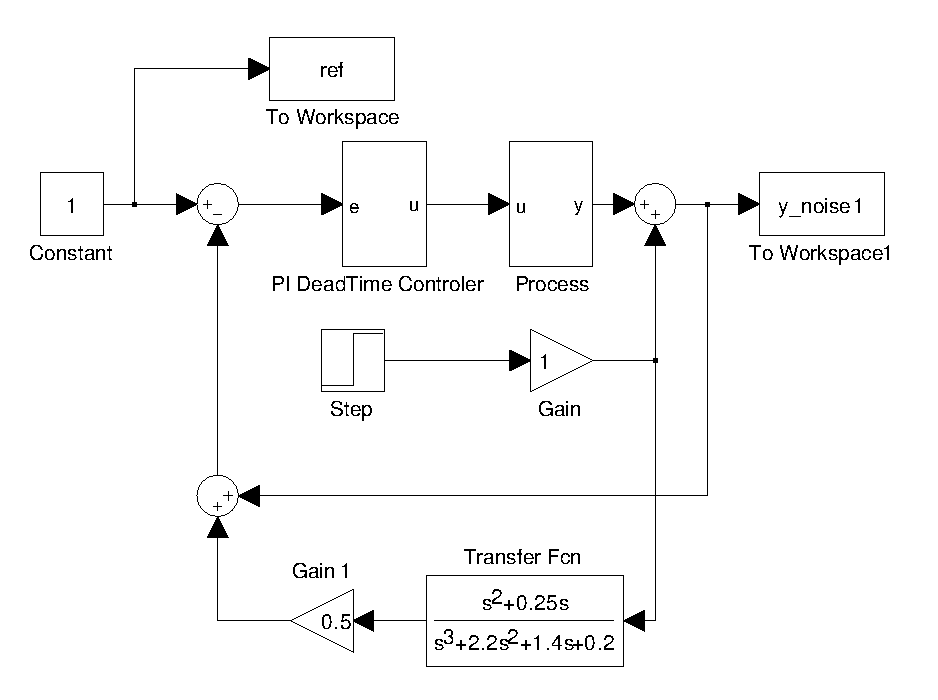
\includegraphics[width=0.75\textwidth]{imgs/questao4/sist_ruido_ff1}
\caption{Sistema com ruído na saída com compensação {\it feedforward} 
         $G_{\text{ff}_1}$.}
\label{fig:q4:sist_ruido_ff1}
\end{figure}

\begin{figure}[H]
\centering
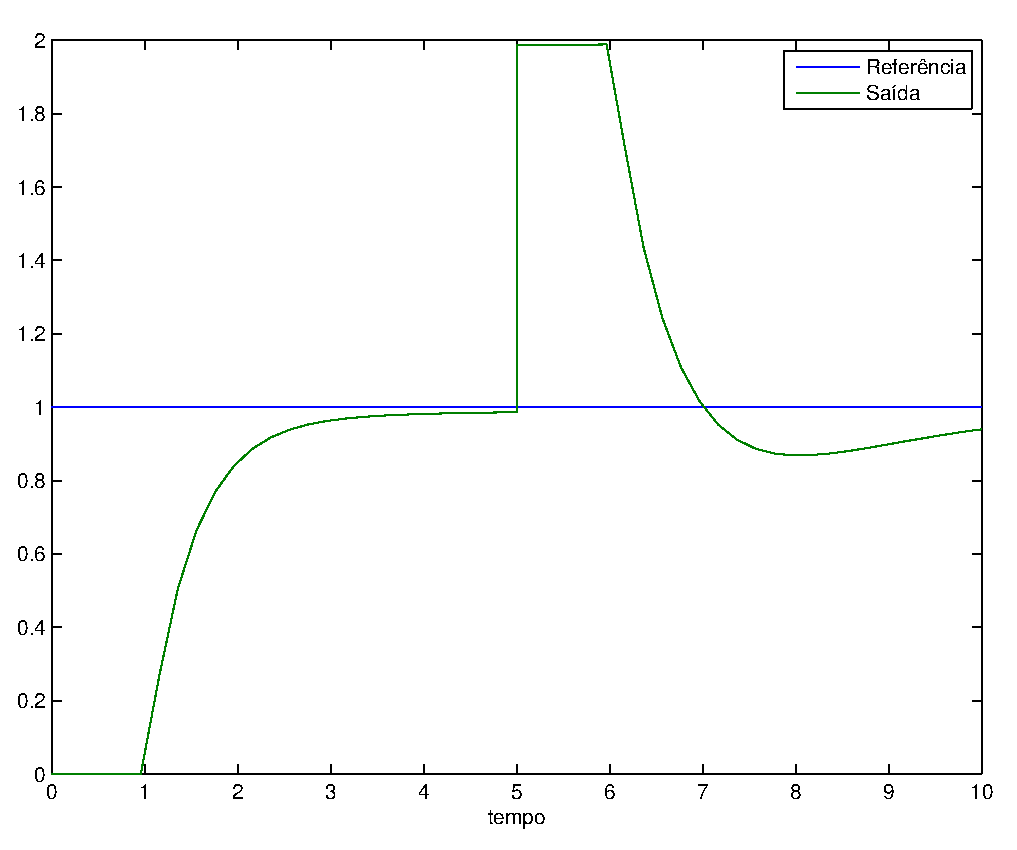
\includegraphics[width=0.65\textwidth]{imgs/questao4/saida_ruido_ff1}
\caption{Resposta do sistema da Fig. \ref{fig:q4:sist_ruido_ff1}.}
\label{fig:q4:saida_ruido_ff1}
\end{figure}

\begin{figure}[H]
\centering
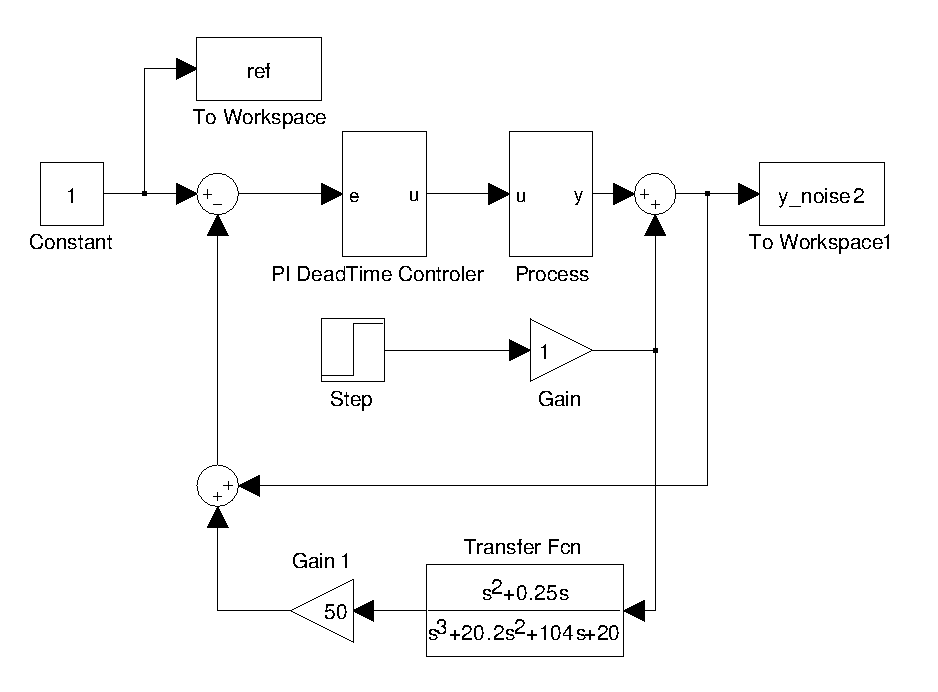
\includegraphics[width=0.75\textwidth]{imgs/questao4/sist_ruido_ff2}
\caption{Sistema com ruido na saída com compensação {\it feedforward}
         $G_{\text{ff}_{10}}$}
\label{fig:q4:sist_ruido_ff10}
\end{figure}

\begin{figure}[H]
\centering
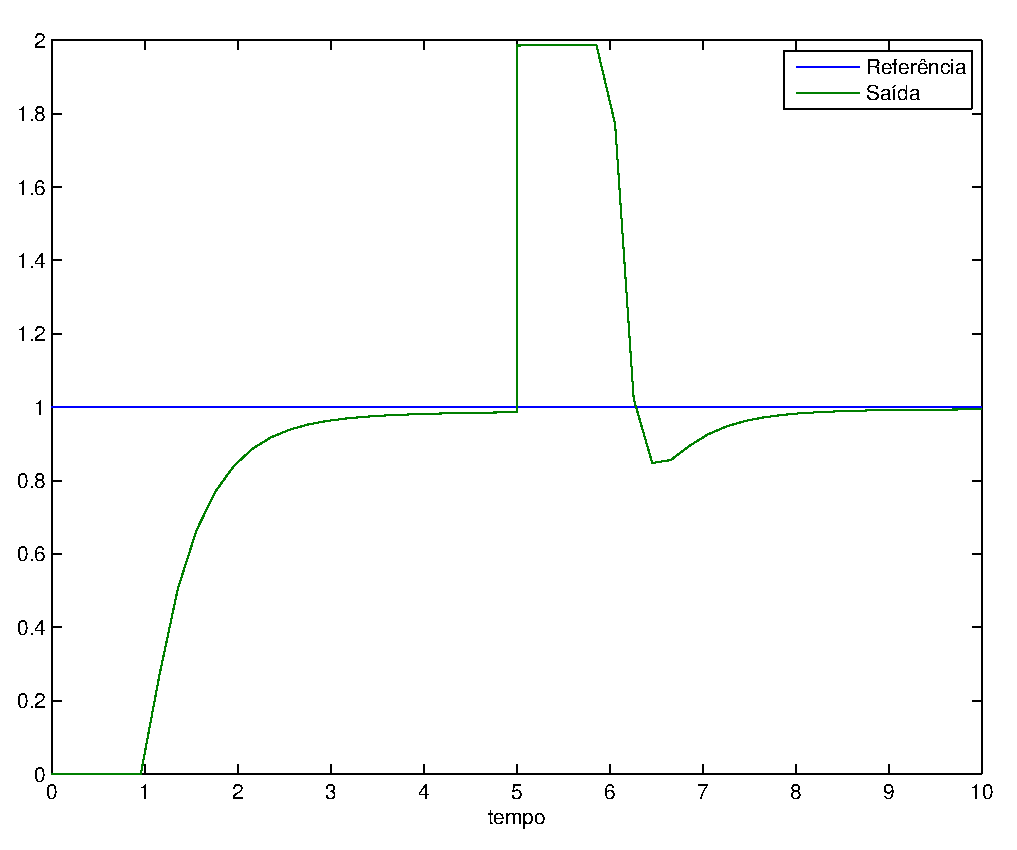
\includegraphics[width=0.65\textwidth]{imgs/questao4/saida_ruido_ff2}
\caption{Resposta do sistema da Fig. \ref{fig:q4:sist_ruido_ff10}.}
\label{fig:q4:saida_ruido_ff10}
\end{figure}

Observando-se o resultado dos três sistemas nota-se que, nesse caso, apesar do
que o próprio nome sugere, o controle {\it feedforward}, não irá atuar
antecipadamente em relação ao controle PI já instalado, pois, já que o distúrbio
atua instantaneamente na saída, o sinal de erro por ele gerado é detectado
(também instantaneamente) pelo controlador PI (com preditor) já instalado. Por
essa razão o sinal de saída do sistema sem o controle FF não se diferencia muito
em termos de desempenho dos sistemas com controle {\it feedforward}.

No entanto a adiçãoda compensação FF, possui uma diferença básica, a rapidez da
reação ao ruído após o tempo $t_r + \tau$, ou seja, passado o intervalo do
atraso de transporte após a aplicação do ruído, como pode ser visto na Fig.
\ref{fig:q4:saida_ruido_ff10}, na qual há um sobressinal na compensação do
ruído. Esse comportamento é devido à excitação do controlador $G_c(s)$ não
somente pelo erro gerado pelo ruído mas também sinal proveniente de
$G_\text{ff}(s)$ e possui a característica de causar um sobressinal no
restabelecimento da referência. A reação ao ruído na Fig.
\ref{fig:q4:sist_ruido_ff1}, no entanto, é bastante lenta, devido aos dois
filtros $F_1(s)$ utilizados, por possuírem uma constante de tempo elevada
($1$), apresentando o pior desempenho entre os três.
